\documentclass[11pt,a4paper]{article}
%\usepackage[toc,page]{appendix}
\usepackage{graphicx}
\usepackage[a4paper]{geometry}
\usepackage{xcolor}
\usepackage{fancyhdr}
\usepackage{float}
\usepackage{setspace}
\usepackage[absolute]{textpos}
\usepackage{epstopdf}
%\usepackage[]{mcode} 	% To include matlab code
\usepackage{capt-of}
\usepackage{enumerate}
\usepackage{lastpage}
\usepackage{booktabs}
\usepackage{longtable}
\usepackage{array}
\renewcommand{\arraystretch}{1.5}

\usepackage[english]{babel}
\usepackage[utf8]{inputenc}
\usepackage{amsmath}
\usepackage{amsfonts}
\usepackage{graphicx}
\usepackage[colorinlistoftodos]{todonotes}
\usepackage{algorithm}
\usepackage{algpseudocode}

\usepackage{amsmath}
\usepackage{algorithm}
%\usepackage[noend]{algpseudocode}
\makeatletter
\def\BState{\State\hskip-\ALG@thistlm}
\makeatother

\usepackage{amsmath}
\usepackage{amsfonts}
\usepackage{amssymb}
\usepackage{eurosym}

% Header
\setlength{\headheight}{30pt}
\newgeometry{top=2.5cm, bottom = 1.5cm, left=2cm, right=2cm}
\pagestyle{fancy} 
\lhead{\includegraphics[height=0.8cm]{figures/{tue_logo}.png}}
%\lfoot{Group 4 - ``CASE"-HENK}
\cfoot{~}
\rfoot{Page \thepage ~of \pageref{LastPage}}

\usepackage{cleveref}
% Change cleveref reference eq. to equation same for figure
\crefname{equation}{equation}{equations}
\crefname{figure}{figure}{figures}
\crefname{table}{table}{tables}

% Change Section numbering to Problem 1
%\renewcommand{\thesection}{Problem \arabic{section}.}

\begin{document}
%\begin{titlepage}
%\vspace*{100pt}
%\begin{figure}
%\centering
%\includegraphics[width=0.5\textwidth]{figures/TUelogozondertekst}
%\end{figure}
%\begin{center}
%{ \huge \bfseries 4AT100 Automotive Systems Engineering Project\\[0.4cm] }
%\textsc{\Large Concept Project Plan}\\[0.5cm]
%
%\end{center}
%
%\vfill
%
%\renewcommand{\arraystretch}{1}
%
%\begin{flushleft} \large
%\begin{tabular}{l}
%Project Coordinators:\\
%Dr.Ir. A. van de Mortel-Fronczak (Asia) \\
%Dr.Ir. I. Barosan (Ion) \\
%\end{tabular}
%\end{flushleft}
%
%\begin{flushleft} \large
%\begin{tabular}{l l l l}
%Tutor: & & & \\
%L. Kefalidis (Lazaros) & & & \\
%& & & \\
%Authors:\hspace{30mm} 	& \hspace{35mm}	& \hspace{55mm} 	    		& 			\\
%S. Forno (Simone) 		& ​0978942		& T. de Mor\'ee (Tim)			& 0944052 	\\
%R.M.A. Goris (Rob) 		& 0808822		& T.M.A. van de Wiel (Thijs)	​& 0824530 	\\
%B.S. Haarsma (Bouke) 	& 0751757​		& H. Wils (Hielke) 				& 0807014 	\\
%\end{tabular}
%\end{flushleft}
%
%\begin{flushleft} \large
%\begin{tabular}{l}
%MSc. Programme Automotive Technology \\
%Eindhoven University of Technology \\
%\end{tabular}
%\end{flushleft}
%
%\begin{flushleft} \large
%\begin{tabular}{l}
%\today \hspace{8.4cm} Group 4 ``CASE"-HENK \\
%\end{tabular}
%\end{flushleft}
%
%\renewcommand{\arraystretch}{1.5}
%
%\end{titlepage}

\newgeometry{top=2.5cm, bottom = 3cm, left=2cm, right=2cm}

%\newpage
%
%\setcounter{tocdepth}{2}
%
%\tableofcontents
%\newpage


%------------------------------------------------

\section{Results}

About the wireless plugin, there was an evaluation error, according to the comment seen here: http://answers.gazebosim.org/question/13021/plugin-for-wirelesstransmitter-and-wirelessreciever-sensors/. In this blog, the Wireless plugin happens to be within Gazebo7, however this doesn't mean we have to use Gazebo7. 

The nice thing would be to have a $prebuilt$ WirelessPlugin (a file with $.so$ extension), ready to use in the Gazebo simulation. To do so:
\begin{itemize}
\item Find a robot in Kinetic with a Wirelessplugin, perform the installation via sudo-apt-install-kinetic-'name of the robot'
\item Restore the old situation of the simulation so far, but with the new robot
\end{itemize}

Notes: Remember when you start a new clean catkin-ws, the file $bashrc$ should be completed as follows. Add the following lines to the file:
\begin{itemize}
\item /opt/ros/ros-distro/setup.bash
\item tildasymbol/catkin-ws/devel/setup.bash
\item export ROS{\_}PACKAGE{\_}PATH=/home/yourname/catkin{\_}ws/src:ROS{\_}PACKAGE{\_}PATH
\end{itemize}

Now I was trying to see if the AGV robot (wiki.ros.org/agvs) which is not an official installation of Hydro, can be compiled into the Kinetic release. The Gazebo is working, but the control not. The gmapping and amcl are working, so now try to make the Husky working too.

The big challenge is, and it would be nice to have, find a robot with Wifii to be installed directly into Kinetic and be simulated here.


\section{To do`s} \label{sec:todos}

\begin{itemize}
\item Install $gazebo$ $ros$ $packages$ or similar and check it on a Kinetic robot (try with the Husky distro found for Kinetic) and install the corresponding packages ------ search for something like "How to install gazebo-ros-pkgs for Kinetic"
\item How to have a direct .so file for Wirelessplugins? Probably need to write one myself
\item \textbf{Pose the question on Wiki.Ros.questions !!}
\item Add an antenna model receiver onto the Husky URDF description, passages are on Section \ref{sec:plugin_tutorials}.
\item Look into the Transmitter propagation model and understand the basic principle of it. The variable \textbf{ModelStrdDevs, represents the st.dev of the Gaussian propagation model}
\end{itemize}

\section{Achieved}

\begin{itemize}
\item Plugins are neither installed with the ROS distro (Kinetic, Indigo, ..) nor with the robot itself. They are under the folder /devel/lib and they come with the $gazebo$ $ros$ $packages$. It is possible that the .so file came from a catkin-make of some packages, since according to wiki.ros.org/catkin/Tutorials/using-a-workspace the catkin-make writes libraries in to the \textbf{/devel} folder. \textbf{Plugin shared objects found: They come with the gazebo-ros-pkg catkin-make installation, following the tutorial}. If we see inside how the gazebo-ros-pkgs are made we see .cpp and .h files, then by building them with catkin-make. Additional note is, according to the official Gazebo plugin tutorials the available plugins in the folder \textbf{gazebo-plugins} are found also under the path: /opt/ros/kinetic/include/gazebo-plugins, in form of header files .h
\item On the Ubuntu 14.04 the Indigo system has been completely reinstalled
\item The gazebo-ros-pkgs successfully build and the .so files are placed under the /devel folder. Since the Wirelessplugins was missing, I cloned the Gazebo master release which contains the wireless sensors .cpp and .h files, add them into the gazebo-plugin source folder, built them with catkin-make to check if the .so files libraries are added into the \textbf{simone-ws/devel/lib}, however \textbf{no Wireless.so file has been automatically created}. This implies some modifications into the .cpp and .h single plugin files maybe
\item Husky packages have been restored in the Kinetic distro, the simulation is again at the last point in time left on the 20.Aug.
\item  The antenna receiver is now on the Husky robot, under the additional folder
\end{itemize}

\section{Notes on Wifii Plugin implementation} \label{sec:Plugins}

\subsection{Notes on Plugins tutorials} \label{sec:plugin_tutorials}

A small document with a review of the xacro and macro properties of the Husky is available in the Ubuntu PC of KFS; the receiver model has to be moved onto the husky robot, and the plugin should be wrapped into the robot as well. Maybe a physical model is actually not needed, but just insert the sensor tag i.e. sensor tag symbol, with the corresponding properties.

Adding a wireless receiver as an small cylinder antenna, modifying the Husky URDF. xacro files. 
As first according to the Clearpath robotics following the Customized Husky config, the \textbf{husky-customization} folder has been cloned. This contains two subfolders, the husky-custom-description and the husky-custom-gazebo, and since we want to add an URDF element onto the Husky, we directly use the first subfolder. The file \textbf{custom-description.urdf.xacro} has been modified with the Receiver link and joint of the Wireless Receiver (simple white cylinder anternna). In order to make it work, the $description.launch$ file include file is added with the custom.urdf.xacro file. 

\vskip 0.2cm

Now the WirelessReceiver has to be fired up and added as a sensor tag into the custom.urdf.xacro file. At this time I am first following the \textbf{http://gazebosim.org/tutorials?tut=ros-plugins} tutorial. The aim is to make a shared object file (.so) to add into the custom.xacro file of the Husky.

\subsection{The single Receiver and Transmitter .cpp and .h files}

Taken the file $gazebo-ros-laser cpp$ it is visible that a node is created, which advertises (i.e. publishes) data on a pre-created message, in this case the sensor-msgs:LaserScan. It is very likely that the Transmitter plugin should do the same.

\vskip 0.2cm

The class reference for the WirelessTransmitter and Receiver plugins are found under \textbf{http://osrf-distributions.s3.amazonaws.com/gazebo/api/2.2.1/classgazebo{\_}1{\_}1sensors{\_}1{\_}1WirelessTransmitter.html}



\subsubsection{WirelessTransmitter}

Description of the Transmitter by function block

\begin{itemize}
% \item In the constructor class definition, there is a \textbf{frequency} tag specified
\item The constant NObstacle has been placed to \textbf{0}, no ostacles present between the transmitter and the receiver
\item On \textbf{Line 39} the WirelessTransmitter class is wrapped with a Transceiver class, what is the role of the Transceiver? The \textbf{GetTopic} function is defined in the Transceiver.cpp on line 46
\item \textbf{void WirelessTransmitter::Load(const std::string \&{\_}worldName)} there is a reference to a worldModel. As in the Section 4.2.3 it checks for the transceiver element.

\textbf{On line 72} the publisher \textbf{pub} is used to publish the propagation model data, publishing data on the msgs::PropagationGrid, gets the topic with Gettopic() function define in the Transceiver model, on \textbf{line 127} it publishes the PropagationGrid msg object
\item \textbf{void WirelessTransmitter::Init()} the testRay is used to check collision between obstacles in the \textbf{GetSignalStrenght} function.
\item \textbf{bool WirelessTransmitter::UpdateImpl()} this is where the propagation model is defined and where the signal $strenght$ is calculated. An object \textbf{msg} is defined with the type $PropagationGrid$, this will later be published. \textbf{Need to understand the propagation model}. On line \textbf{127} the \textbf{pub} publishes the propagation model via the \textbf{msg} tag, but wouldn't be the msg empty?
\item The functions \textbf{GetESSID} and \textbf{GetFreq} are self-explaining
\item \textbf{double WirelessTransmitter::GetSignalStrength(const math::Pose \&{\_}receiver,const double rxGain)}, this function takes as input the \textbf{receiver} via its reference \& and the \textbf{rxGain i.e. the receiver gain}, constructs a 3-Dm vector from the sensor position to the end of the receiver. On \textbf{Line 178} a $distance$ is calculated as the max (std::max) between 1 (?) and the referencePose.pos.Distance({\_}receiver.pos), I think the distance between the sensor and the receiver, then the \textbf{wavelenght} is calculated, then it returns \textbf{rxPower}

\end{itemize}

\subsubsection{WirelessReceiver}

Description of the Receiver by function blocks

\begin{itemize}
\item The function \textbf{void WirelessReceiver::Load(const std::string \&{\_}worldName)}, with \textbf{pub} publishes the propagation model and the corresponding node with message type \textbf{msgs::WirelessNodes}, gets the \textbf{transceiver element} like in Section 4.2.3
\item \textbf{bool WirelessReceiver::UpdateImpl(bool)} is also present in Section 4.2.1 for the Transmitter, defines a \textbf{msg} object of the type \textbf{msgs::WirelessNodes}, defines \textbf{rxPower, this is the return of GetSignalStrenght function} and a \textbf{txFreq, transmitter frequency acquired in Line 113}, get the sensors in the SDF file via GetSensors(), line \textbf{108} checks for "wireless{\_}transmitter", in Lines \textbf{114 and 115} take via the functions GetFreq and GetSignalStrenght the transmitter and \textbf{freq} and \textbf{power}, what does this do \textbf{msgs::WirelessNode *wirelessNode = msg.add{\_}node()?}



\end{itemize}

\subsubsection{WirelessTransceiver}

Description of the Transceiver by functions blocks

\begin{itemize}
\item The \textbf{GetTopic} function is defined in the Transceiver.cpp on line 46 and is used in the Transmitter and Receiver models to get the topic name from the SDF files
\item In the function of line 56 \textbf{void WirelessTransceiver::Load(const std::string \&{\_}worldName)} the $reference-pose$ takes in the sensor reference pose (think defined under the sensor SDF tag `pose`) while the $pose$ the sensor pose (Have no clue which is the difference). Then the $parent-entity$ helps preventing the dynamic cast. Formula : ref pose = pose + parent entity.
On line 67 checks for a missing Transceiver element, this is present in the $\langle$transceiver$\rangle$ tag of the MLR-Arena model. Gets the transceiver element with \textbf{sdf::ElementPtr transceiverElem = this->sdf->GetElement("transceiver")}
The \textbf{Lines 73 and 74} gets the \textbf{gain} and \textbf{power} elements.
\item The function \textbf{GetPower} and \textbf{GetGain} return the power and gain previously acquired
\end{itemize}



\subsection{Steps taken and tentatives to fire up the WirelessPlugin}

These are the tentatives to fire up the WirelessTransmitter and WirelessReceiver plugin: 



\subsection{Question - Gazebo answers}

Formulation of the question of the Gazebo ROS.
The main idea is to fire up a Transmitter plugin on the Husky robot, which broadcast some sort of wireless signals over the simulation or directly to a fix Receiver, that receives the signal or listens to it over the simulation

The main guiding questions:
\begin{itemize}
\item Where to place the .cpp and .h files to fire up the plugin and create the library file?
\item How does the communication between the two tags works? 
\item On which topic should the plugin publish to?
\end{itemize}



\end{document}






% == TABLE ==
%begin{table}[h!]
 % \centering
  %\caption{Caption for the table.}
 % \label{tab:table1}
 % \begin{tabular}{ccc}
 %   \toprule
  %  Some & actual & content\\
   % \midrule
   % prettifies & the & content\\
   % as & well & as\\
  %  using & the & booktabs package\\
  %   \bottomrule
  %\end{tabular}
%\end{table}


% === ALGORITHM == 

\iffalse % multi-comment tool
\begin{algorithm}[!h]
   \caption{Kirsch, Rohig algorithm}
    \begin{algorithmic}[1]
    	\State $St-1 = St$
        \For{$i = 1$ to $N$} \Comment{With N the number of particles in the filter set by maxparticle parameter}
            \State $Spread $ $particles$ $in$ $the$ $anchorbox$ $with$ $equations$ $1)$ $and$ $2)$ $of$ $[3]$ \Comment{This step is called $Global$ $Localization$}
            
            \State $xt[n] = p(xt|xt-1,ut)$ \Comment{Motion update - sample the particles from the motion update of the robot and move forward to estimate the error model functions}
            
        	\State $wt[n] = p(dnanoLOC|si)*p(dlaser|si)$ \Comment{Measurement update - si are the particles set with i the i-th index}
        	\State $St = St + <xt,wt>$ \Comment{add the state and weight to the total state space}
        	
        	\State $Perform$ $resampling$
        \EndFor
    \State $Return$ $St$

\end{algorithmic}
\end{algorithm}
\fi


\iffalse

\begin{figure}[!htb]
    \centering
    \begin{minipage}{.5\textwidth}
        \centering
        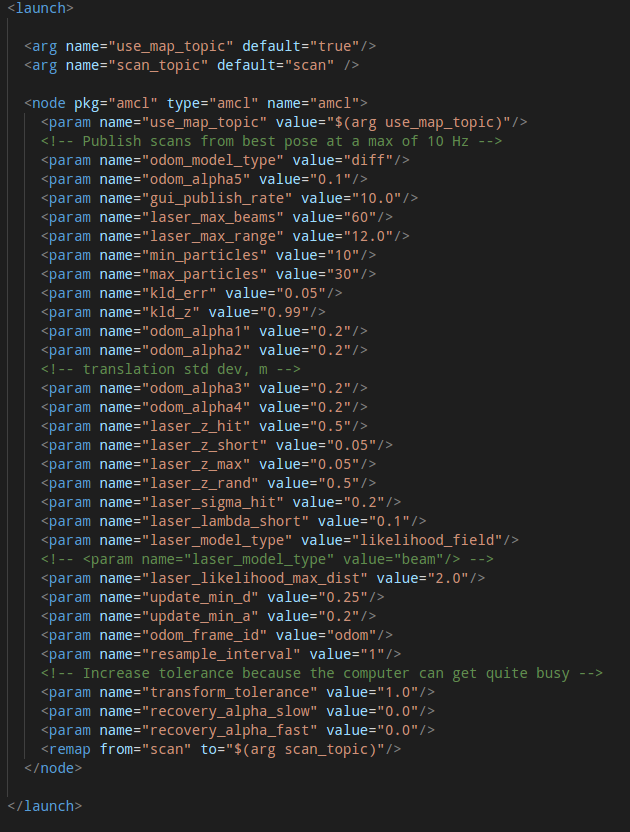
\includegraphics[width=0.7\linewidth, height=0.2\textheight]{figures/amcl_param}
        \caption{The $amcl$ tunable parameters}
        \label{fig:amcl_param}
    \end{minipage}%
    \begin{minipage}{0.5\textwidth}
        \centering
        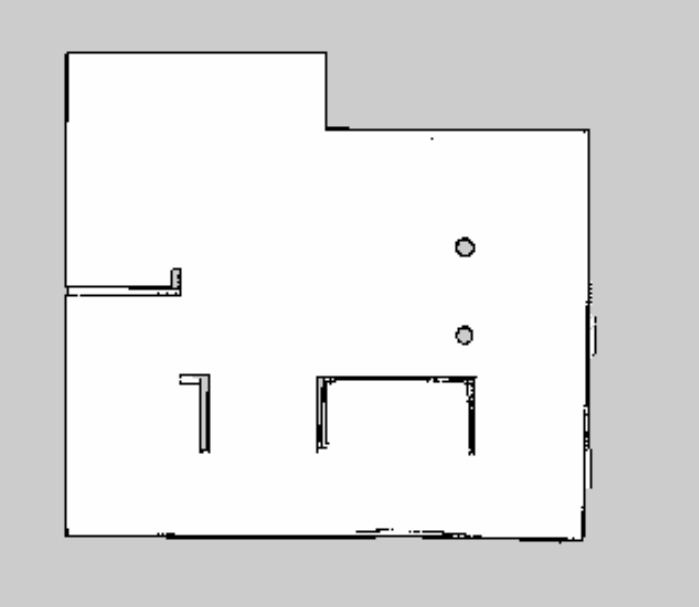
\includegraphics[width=0.7\linewidth, height=0.2\textheight]{figures/my_amcl_gmapping}
        \caption{Result of the Gmapping for the simple indoor environment}
        \label{fig:myamcl_map}
    \end{minipage}
 \end{figure}
 
 
 
 \begin{figure}[!htb]
	\center
	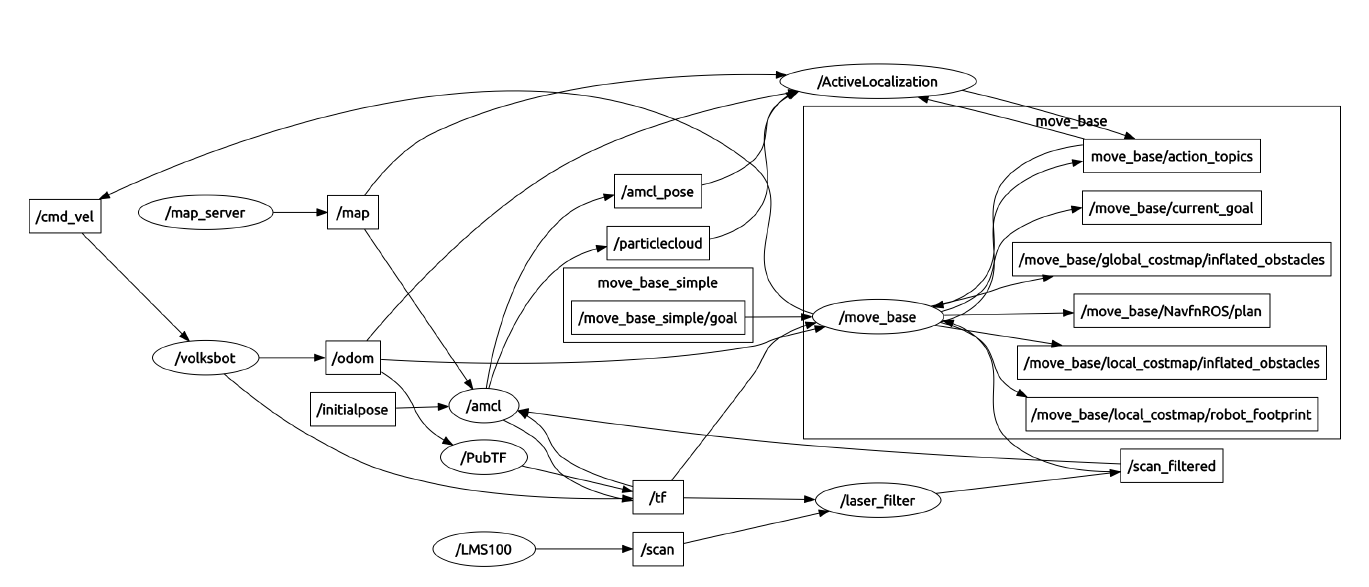
\includegraphics[width=1\textwidth]{figures/active_localization_node.png}
	\caption{An example of an active localization node}
	\label{fig:active_locnode}
\end{figure}

\fi